\chapter{Benchmarking Case Study Implementations}
Now that we have the two implementations, we wish to define a workflow that'll be used to benchmark them. The workflow should be deterministic, so we can recreate its exact form for each implementation, and scalable, so we can steadily increase to see how each version compares to increased load.
\section{Workload}
We've defined syncers that sync a single product across two services. We can say that a workload is syncing all products. That means we have to generate the appropriate resources on each service. This raises the question: for a product on the PS store, which are the possible states on the online store? For any product on the PS store it can either (a) be fully synced on the online store, (b) be partially synced or (c) not exist at all on the online store. In other words, a workload of X products, some of them should be in the (a) state, other on the (b) and the rest on the (c) state. A Pseudo-Random Number Generator (PRNG) can be used for generating the data, as well as the number of models on the states mentioned earlier.

Thus, a workload is defined by X, total number of models and S, the seed for the PRNG.
Now, we need to construct a benchmark program that will create workflows of increasing size to measure the performance of each implmentation.
\section{Experimental Setup}
\begin{figure}[h!]
    \centering
    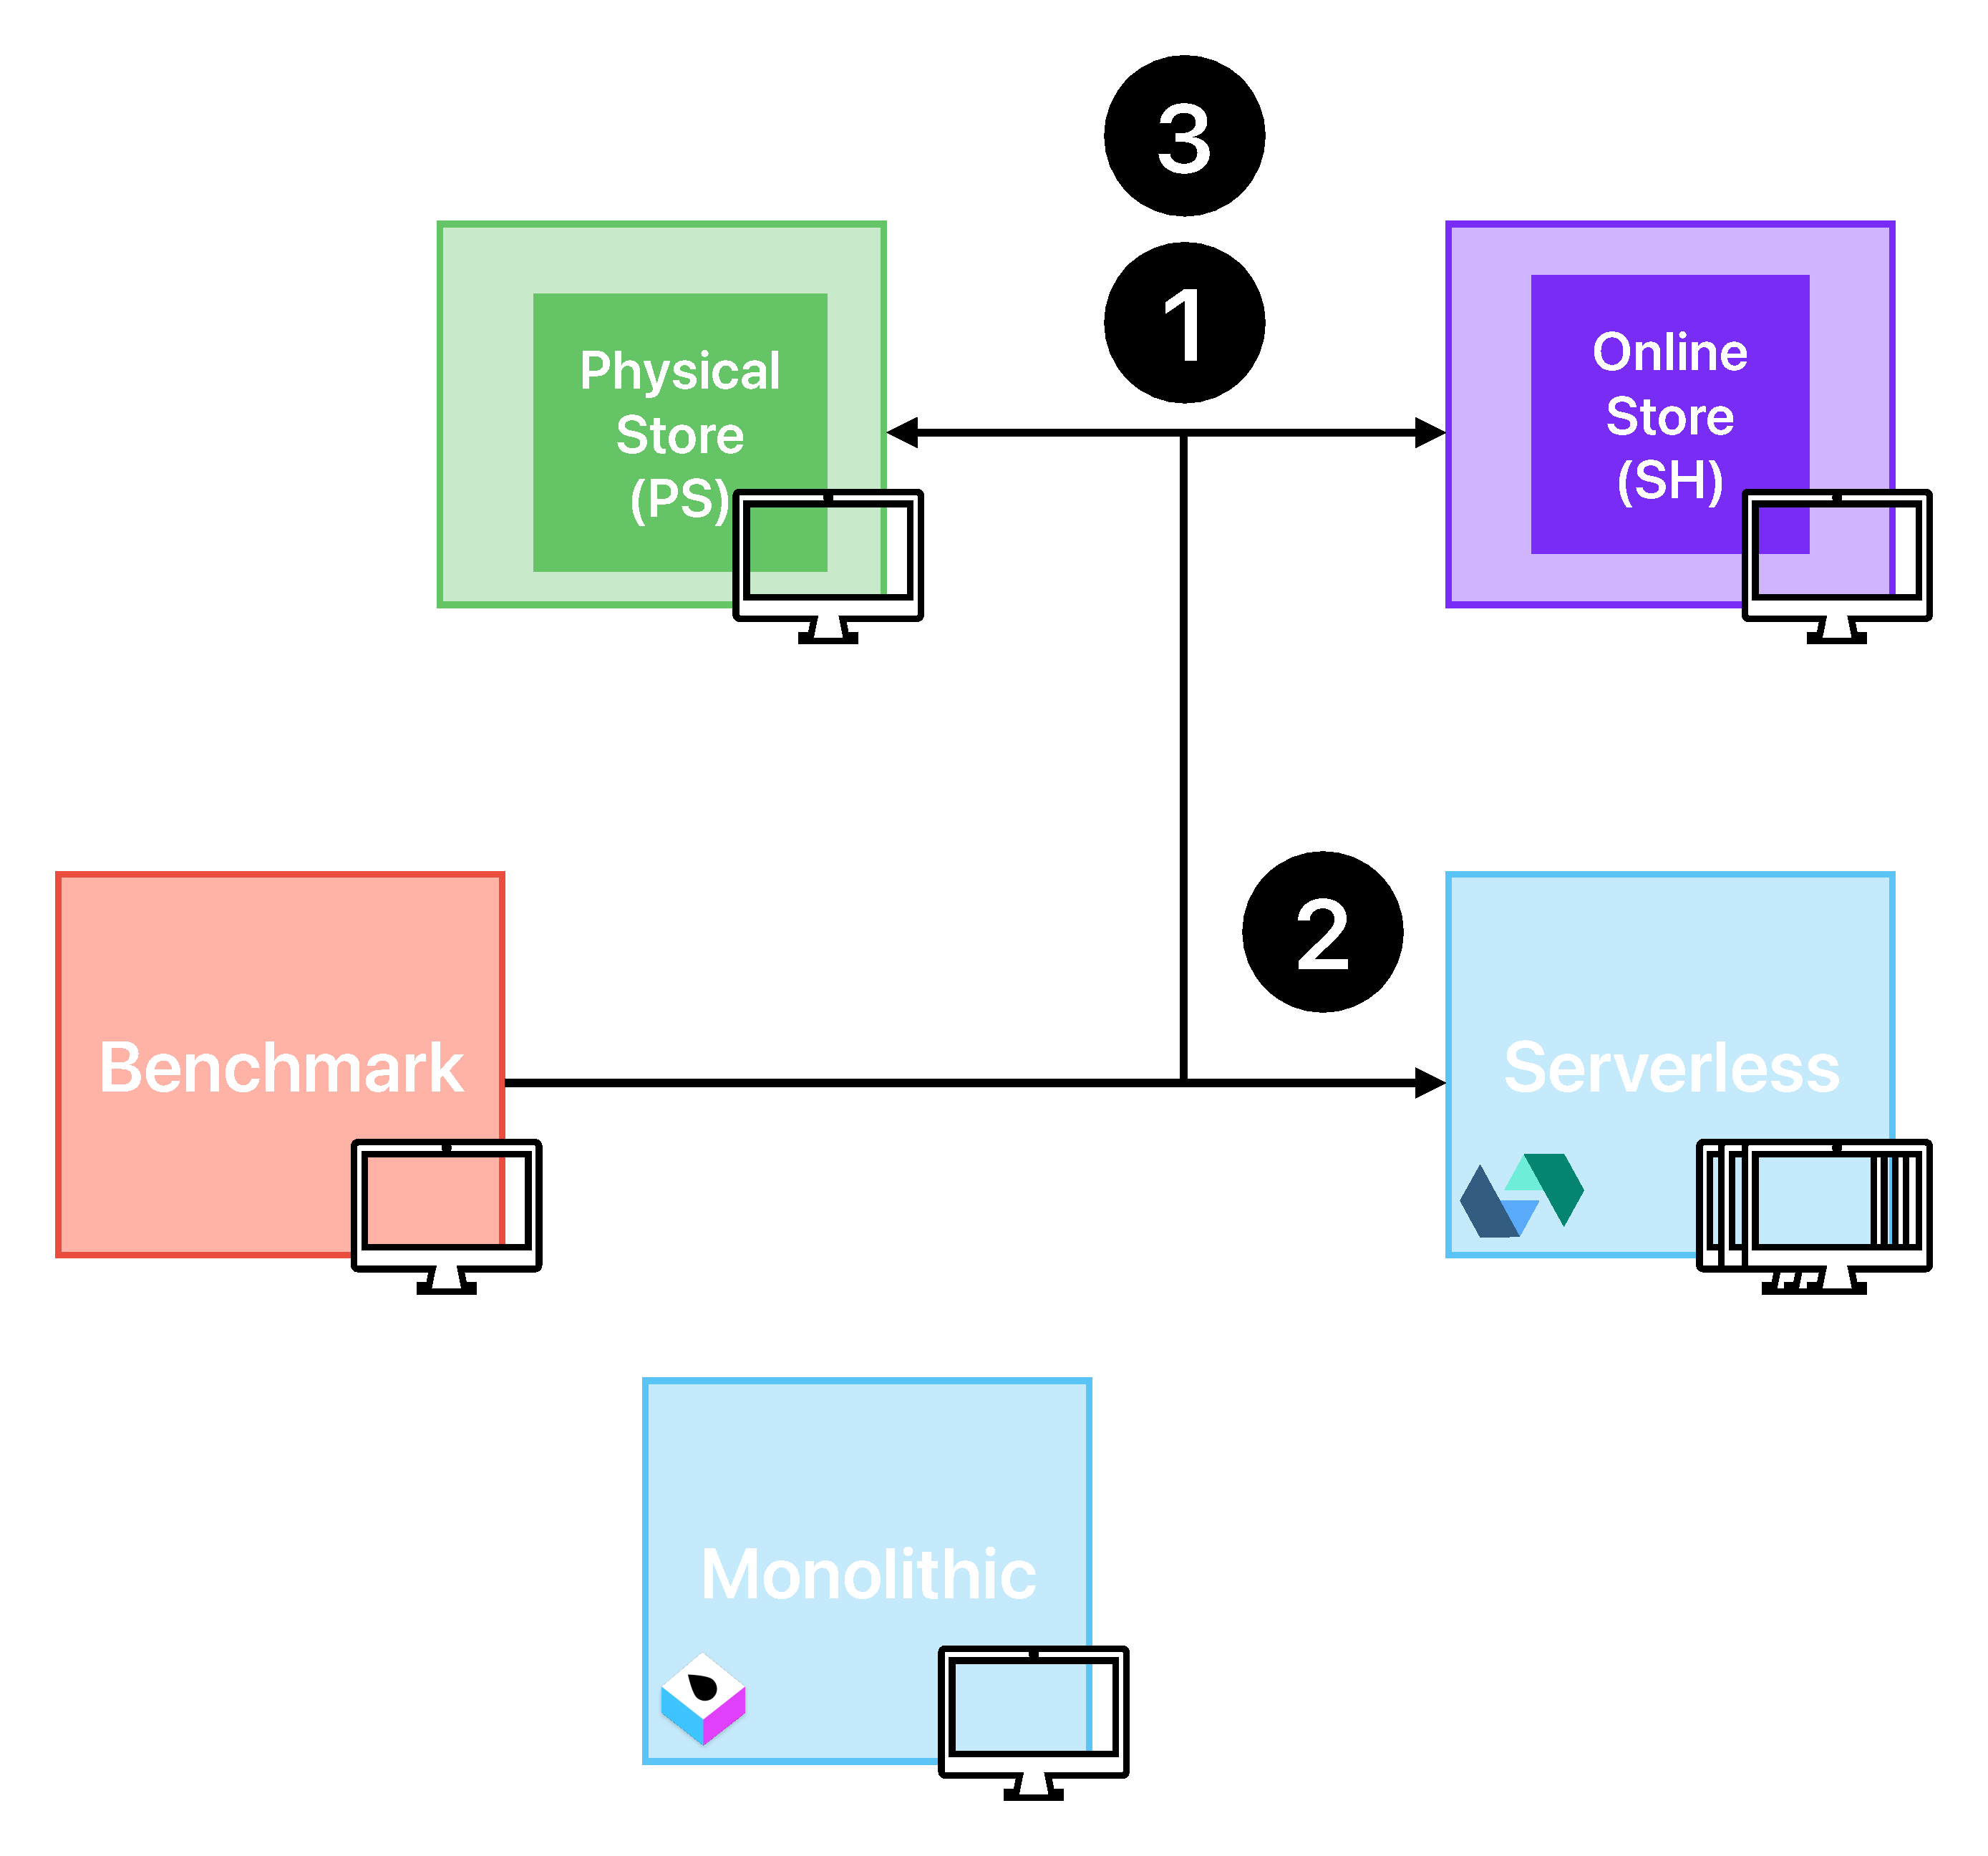
\includegraphics[width=\textwidth]{media/bench_black.pdf}
    \caption{Serverless Deployment}
    \label{fig:sync3_5}
\end{figure}
All the machines used in any experiments are of the same type, m510 on CloudLab. CloudLab is a platform that allows researchers to reserve physical machines for a brief period of time to conduct experiments.

The experimental setup involved deploying the PS and SH servers on separate machines, the monolithic implementation on a single machine. The serverless implementation was deployed on 24 machines, of which 18 are invokers.
In OpenWhisk, machines are either invokers or core nodes. Invokers are machines that actually run the activations. Core nodes are used for everything else, such as Kafka or nginx.
The benchamrk program, for a workload of size X goes through 3 steps for each implementation:
1. Set up the servers: Configure the servers to a state mentioned earlier where some products need syncing.
2. Use the implementation to sync all models
3. Reset the servers, removing all data


\section{Results and Discussion}
In a given workload, sending the model sync request raised the following question: how often should the model sync requests be sent? As the workload increases, should any adjustments be made? As it currently stands, the benchmarker uses Swift's TaskGroup construct to send the requests.
\subsection{Without a Rate Limit}
First, we experimented with leaving it all up to the task group, which resulted in requests being sent roughly all at once. 
\begin{figure}[h!]
    \centering
    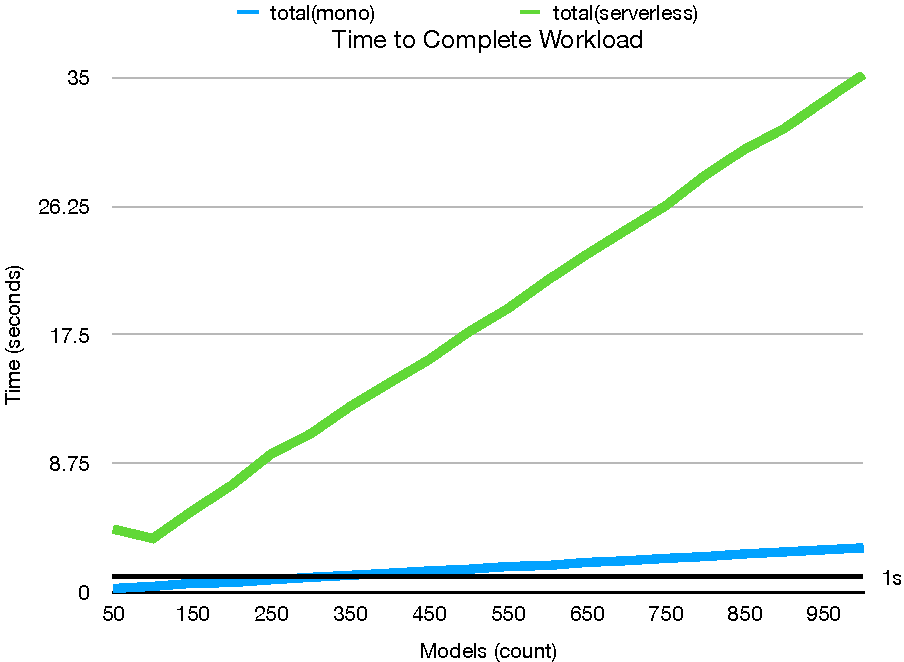
\includegraphics[width=\textwidth]{media/no_rl_ex.pdf}
    \caption{Execution time comparison between serverless and monolithic implementations}
    \label{fig:rate_unlimited_comparison}
\end{figure}
The serverless implementation's execution time increased incomparably to the monolithic version, as seen on figure 5.1.
While for both implementations the median latency did tend to increase, the serverless implementation's latency increased considerably faster, as seen in figures 5.2 and 5.3.
\begin{figure}[h!]
    \centering
    \begin{minipage}{0.48\textwidth}
        \centering
        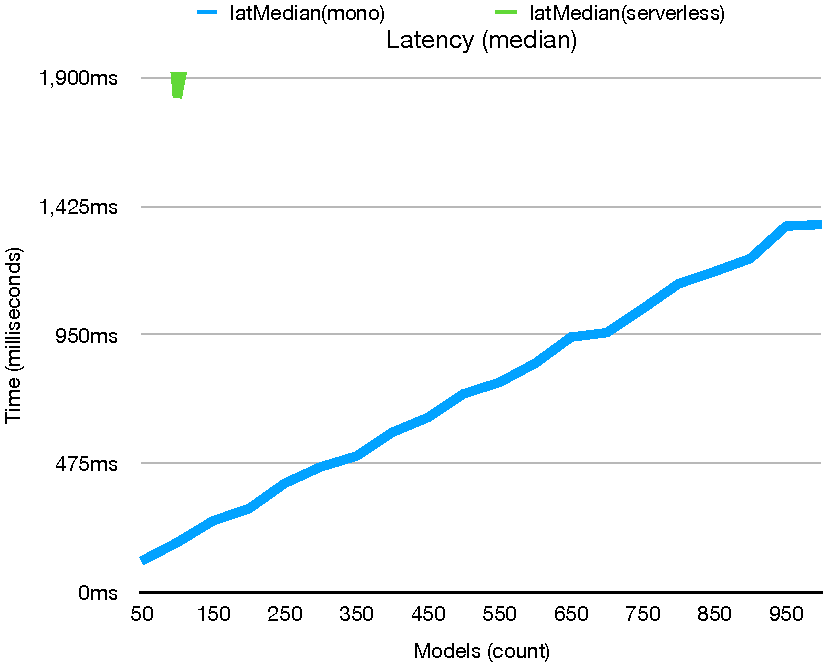
\includegraphics[width=\linewidth]{media/no_rl_mono_lat_med.pdf}
        \caption{Median latency for a single model request, scaled for the monolithic implementation}
        \label{fig:rate_unlimited_comparison_lat_mono}
    \end{minipage}\hfill
    \begin{minipage}{0.48\textwidth}
        \centering
        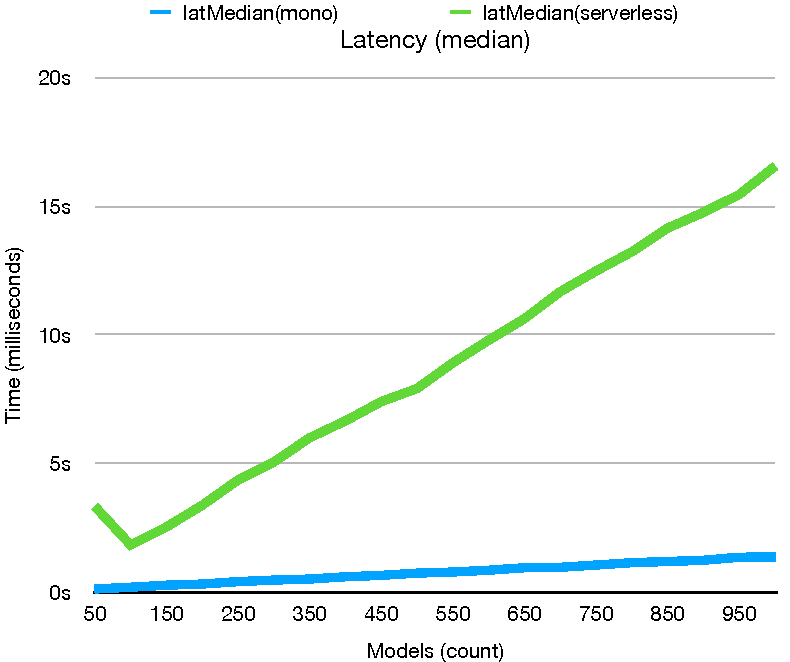
\includegraphics[width=\linewidth]{media/no_rl_lat_med.pdf}
        \caption{Median latency for a single model request}
        \label{fig:rate_unlimited_comparison_lat}
    \end{minipage}
\end{figure}

The above is explained by a much lower Queries per Second (QPS) by the serverless implementation. As seen on figure 5.4, while the serverless implementation seems to have hit a limit of 28 QPS, the serverless implementation seems to hit a limit of 333, more than ten times bigger.
\begin{figure}[h!]
    \centering
    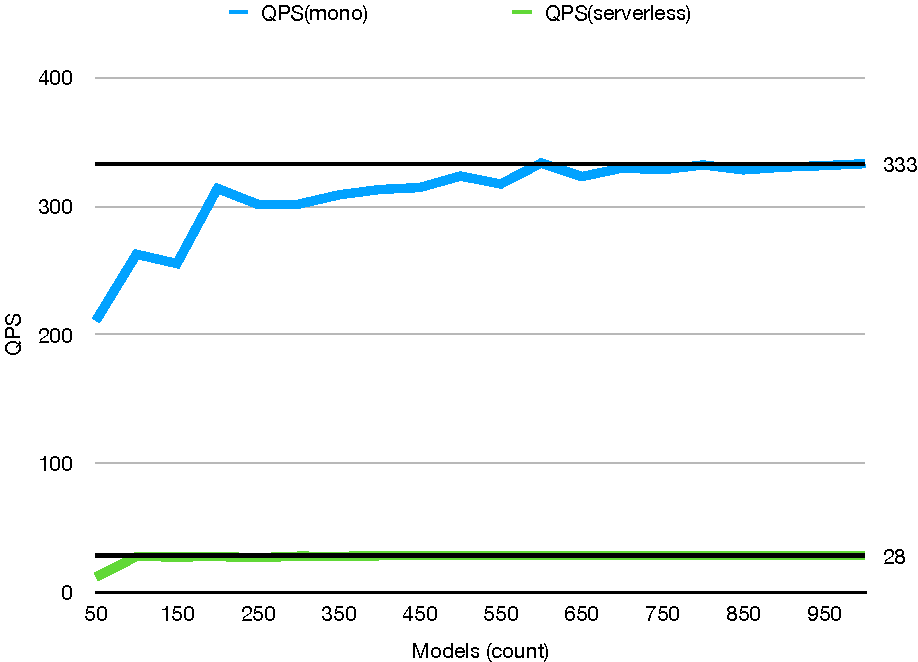
\includegraphics[width=\textwidth]{media/no_rl_qps.pdf}
    \caption{QPS comparison between serverless and monolithic implementations}
    \label{fig:rate_unlimited_comparison_qps}
\end{figure}


\subsection{Implementing a Rate Limit}
We use the Swift Rate Limitter, which is a custom made Swift rate limitter we have developed~\cite{swift-rl}, which is well tested, which allows us to send requests with a minimum set delay between them. We utilized it to send the requests every 100ms. This will cap the maximum QPS to 10 which ensures neither implementation will be stressed, hopefully allowing us to have a clearer picture of the situtation.

With the rate limit both implementations take the same amount of time and bot achieve roughly 10QPS.
As evident from figure 5.5, a single model sync takes roughly 280ms and 60ms on the serverless and monolithic implementations respectively.
\begin{figure}[h!]
    \centering
    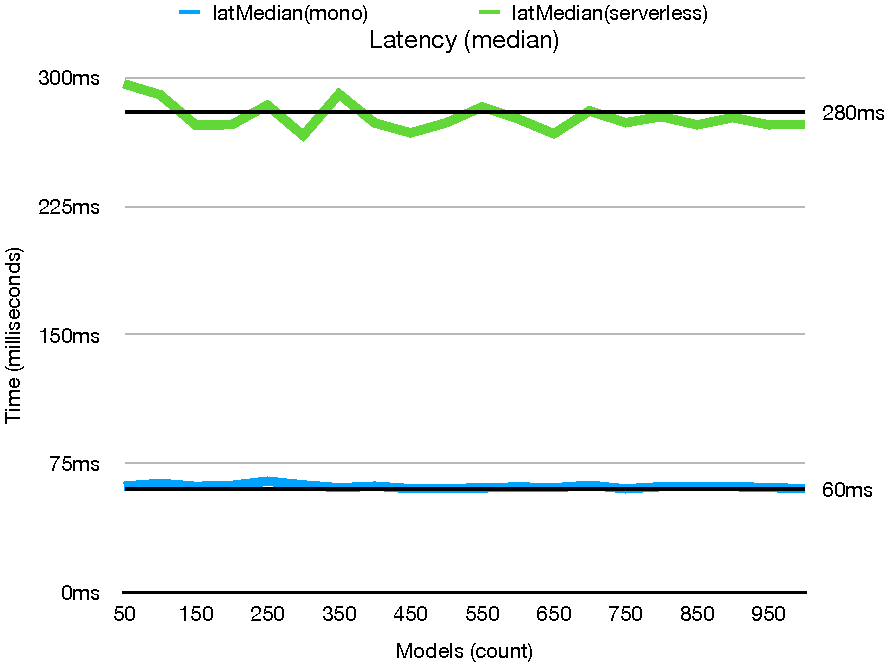
\includegraphics[width=\textwidth]{media/rl100_lat_med.pdf}
    \caption{Rate-limited (100ms) comparison between serverless and monolithic implementations}
    \label{fig:rate_limited_comparison}
\end{figure}
An interesting finding, is that the P99.9\% latency (figures 5.6 and 5.7), apart from being higher, it as less stable on the serverless implementation. This is despite utilizing less than the third of its maximum QPS.
\begin{figure}[h!]
    \centering
    \begin{minipage}{0.48\textwidth}
        \centering
        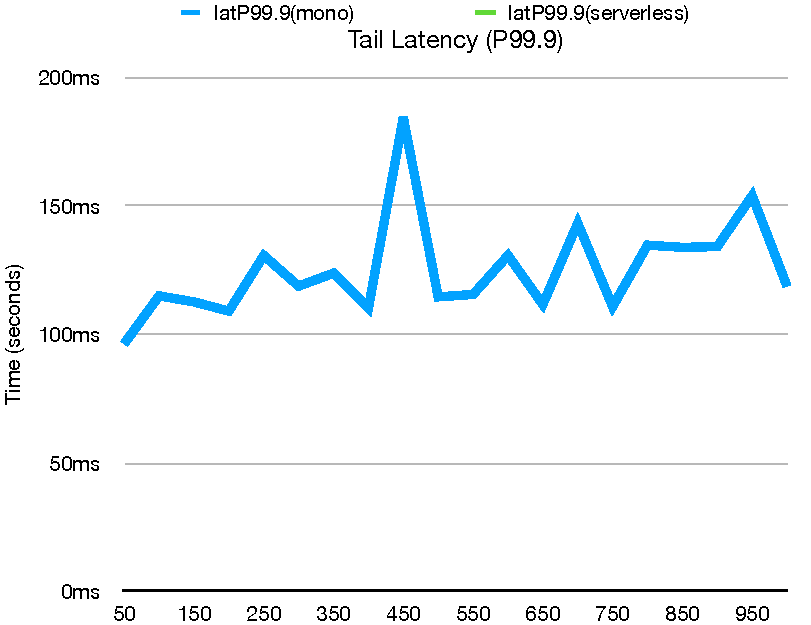
\includegraphics[width=\linewidth]{media/rl100_tl_mono.pdf}
        \caption{Median latency for a single model request, scaled for the monolithic implementation}
        \label{fig:rate_unlimited_comparison_lat_mono}
    \end{minipage}\hfill
    \begin{minipage}{0.48\textwidth}
        \centering
        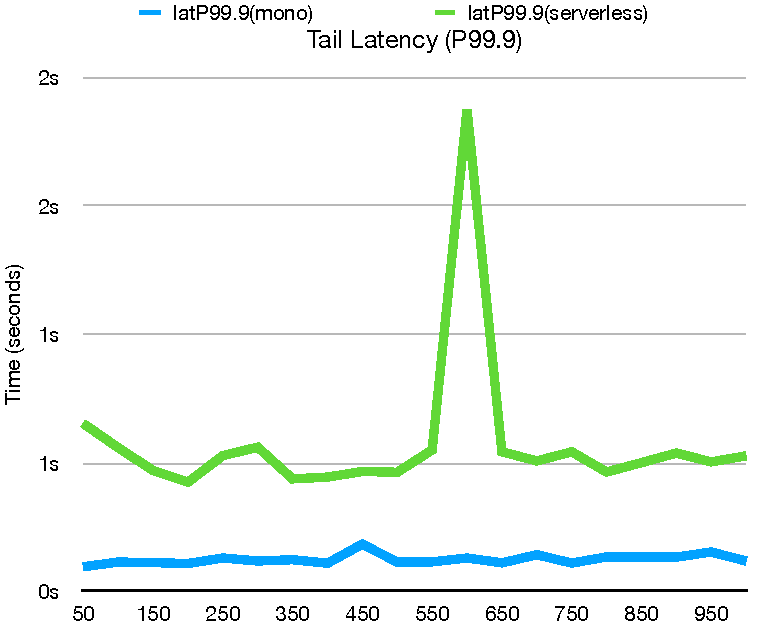
\includegraphics[width=\linewidth]{media/rl100_tl.pdf}
        \caption{Median latency for a single model request}
        \label{fig:rate_unlimited_comparison_lat}
    \end{minipage}
\end{figure}

Despite utilizing 18 machines for executing actions, the serverless approach did not show any clear benefits. This may be attributed to the lack of support for "intra-concurrency" in OpenWhisk runtimes, excluding NodeJS. This limitation significantly affects the scaling capabilities of the serverless implementation, which is a crucial aspect of the serverless or FaaS promise. 18 machines achieving 28QPS means that on average, a request takes 642ms to complete, which is more than double of the 280ms it takes, when the system is not stressed.

\section{Improvements and Future Work}

There are potential avenues for improvement in the serverless system. Notably, updating the Go proxy used by all OpenWhisk runtimes to support intra-concurrency could allow all language runtimes, including Swift, to support concurrent executions, potentially dramatically increasing the maximum QPS.

\section{Conclusion}

The case study findings contribute to the overall conclusion of this thesis, suggesting that the benefit of migrating to a serverless implementation is not always evident and should be carefully assessed for each workflow. The case study also highlights the importance of runtime support for intra-concurrency in realizing the full potential of serverless systems. Without intra-concurrency, the requests stay in memory until a container is available to serve them. The overheads of OpenWhisk may explain the 2 times slowdown of its request completion under load. Notably, the Swift runtime was updated to the latest version to leverage its native async/await features, which played a significant role in the serverless implementation. A total of eighteen identical machines achieving a throughput of ten times less than one single, identical machine is frankly unacceptable. Support for intra-concurrency for the ActionLoop proxy should be a priority for the OpenWhisk project as seamless, efficient scaling is the central promise of FaaS.

